\documentclass[main]{subfiles}
\begin{document}

\section*{Lecture 17 // Oct 20 // Proof of the NST theorem}
\addcontentsline{toc}{section}{Lecture 17 -- Proof of the NST theorem}

\begin{recall}
We defined the $r_s$-invariant for $s\in[-\infty,0]$
\[
r_s(Y) = -\inf_{r<0}\left\{r \mid \exists\ \Theta\text{-supported } [r,-s] \text{ cycle}\right\}
\]
which asks the question ``in which filtered subquotients do we have a cycle of the form $\Theta+\dots$''
\begin{enumerate}
\item $r_s$-invariant is a piecewise constant, non-increasing function.
\item If there exists a negative-definite cobordism $W$ (with $H_1(W)=0$) from $Y_1$ to $Y_2$, then $r_s(Y_1)\leq r_s(Y_2)$. In particular, $r_s$ is a homology cobordism invariant: if $Y$ bounds a negative-definite $4$-manifold $W$ (with $H_1(W)=0$), then $r_s(Y) = \infty$.
\item In addition, if $\pi_1(W)=1$, then the inequality is strict (allowing $\infty\leq\infty$).
\end{enumerate}
\end{recall}

Today, we'll prove one of the main theorems of the NST paper.

\begin{theorem}[NST]\label{thm:nst}
Let $k\subseteq S^3$. Denote $Y_n = S^3_{1/n}(k)$, $n>0$.
\begin{itemize}
\item If $[D_2^{Y_1}]\neq 0$, then none of the $Y_n$ are homology cobordant to each other.
\item If $r_s(Y_1) < \infty$ for any $s$, then $\{Y_n\}_{n=1}^\infty$ is linearly independent in $\Theta^3_{\mathbb{Z}}$.
\end{itemize}
\end{theorem}

\begin{remark}
A-priori, it's not obvious that $\Theta^3_{\mathbb{Z}}$ is at all interesting. For many years after its definition, it was not known whether $\Theta^3_{\mathbb{Z}}$ is $0$, or $\infty$-generated. It is: in particular, it contains a $\mathbb{Z}^\infty$ subgroup ($\bigoplus_{i=1}^\infty \mathbb{Z}_i$). The original proof was due to Furuta and FS in the 80's. In some sense, this theorem is a generalization of theirs. Furuta and FS had the same family, and also used Yang-Mills theory. (Modern language (filtered) allows them to generalize it.)
\end{remark}

\begin{remark}
It's actually very difficult to study $1/n$ surgeries using Heegaard Floer (HF). There's no known invariant coming from HF which distinguishes $\infty$-ly many $1/n$ surgeries on a fixed knot.
\end{remark}

To study linear combinations of $Y_n$, we must first understand the behavior of $r_s$ under $\#$.

\begin{theorem}
For any $s\in[-\infty,0]$ and $s_1,s_2\in[-\infty,0]$ such that $s_1+s_2=s$,
\[
r_s(Y_1\#Y_2) \geq \min\{r_{s_1}(Y_1)+s_2,\ r_{s_2}(Y_2)+s_1\}.
\]
\end{theorem}

Perhaps the form of this theorem -- i.e., it is an inequality, and takes a minimum over a sum of $r_s$'s and $s$'s -- is strange. We'll first give a pseudo-proof of the inequality, since the reason why it's of such a strange form will become apparent during the proof.

\begin{proof}[Proof (sketch)]
We'll pretend that $\underline{C}(Y_1\#Y_2) = \underline{C}(Y_1)\otimes\underline{C}(Y_2)$. This ($\#$ corresponds to $\otimes$) is the behavior one usually expects for complexes under connect sum.

The reducible in $\underline{C}(Y_1\#Y_2)$ is $\Theta_1\otimes\Theta_2$, and $\widetilde{\CS}(\alpha\otimes\beta) = \widetilde{\CS}(\alpha)+\widetilde{\CS}(\beta)$.

Now, fix $s_1$ and $s_2$. Suppose that we have a $\Theta$-supported cycle (a ``OSC'') $\alpha$ for $\underline{C}(Y_1)$ in $[r_1,-s_1]$, and a $\Theta$-supported cycle $\beta$ for $\underline{C}(Y_2)$ in $[r_2,-s_2]$.

What ``$\Theta$-supported'' means is that in $\underline{C}(Y_1)$, $\alpha = \Theta+\dots$. To say that $\alpha$ is a cycle in this subquotient is to say that (a) $\alpha$ is in the subquotient, i.e., $\widetilde{\CS}(\alpha)\leq -s$, and (b) $\widetilde{\CS}(\partial\alpha)<r_1$. In particular, $\partial\alpha$ need not be $0$, but if it isn't, it's outside the subquotient. The same is true for $\beta$: $\widetilde{\CS}(\beta)\leq -s_2$ and $\widetilde{\CS}(\partial\beta)<r_2$.

\textbf{Claim:} $\alpha\otimes\beta$ is a $\Theta_1\otimes\Theta_2$-supported cycle (a.k.a., $\Theta$-supported in the $\otimes$).

We know that $\widetilde{\CS}(\alpha\otimes\beta)\leq (-s_1)+(-s_2)=-s$. So $\alpha\otimes\beta$ is in the subquotient. By the Leibniz rule,
\[
\partial(\alpha\otimes\beta) = (\partial\alpha)\otimes\beta + \alpha\otimes(\partial\beta).
\]
Individually, $(\partial\alpha)\otimes\beta < r_1+(-s_2)$ and $\alpha\otimes(\partial\beta) < (-s_1)+r_2$. Therefore $\alpha\otimes\beta$ is a cycle in the subquotient $\left[\max\{r_1+(-s_2),\ (-s_1)+r_2\},\ -s\right]$. This is where the formula appears.

Now, note that this is true for all $\Theta$-supported cycles in these subquotients. When does this occur? By definition, $-r_{s_1}(Y_1)$ and $-r_{s_2}(Y_2)$ are the borders of when there exists a $\Theta$-supported cycle in each respective subquotient. So the claim is that you can take any $r_1$ up to $-r_{s_1}(Y_1)$ and any $r_2$ up to $-r_{s_2}(Y_2)$. Thus we get a $\Theta$-supported cycle in the subquotient
\[
\left[\max\{-r_{s_1}(Y_1)+(-s_2),\ -r_{s_2}(Y_2)+(-s_1)\},\ -s\right]
\]
\[
\Rightarrow\ r_s(Y_1\#Y_2) \geq \max\{r_{s_1}(Y_1)+s_2,\ r_{s_2}(Y_2)+s_1\}. \qedhere
\]
\end{proof}

\begin{corollary}
$r_0(Y_1\#Y_2) \geq \min\{r_0(Y_1), r_0(Y_2)\}$.
\end{corollary}

To see why this behavior -- taking a minimum instead of adding -- is more natural in this setting, let's do an example.

\begin{example}
Let the following be the $\underline{C}$ complexes for $Y_1$ and $Y_2$.
\begin{center}
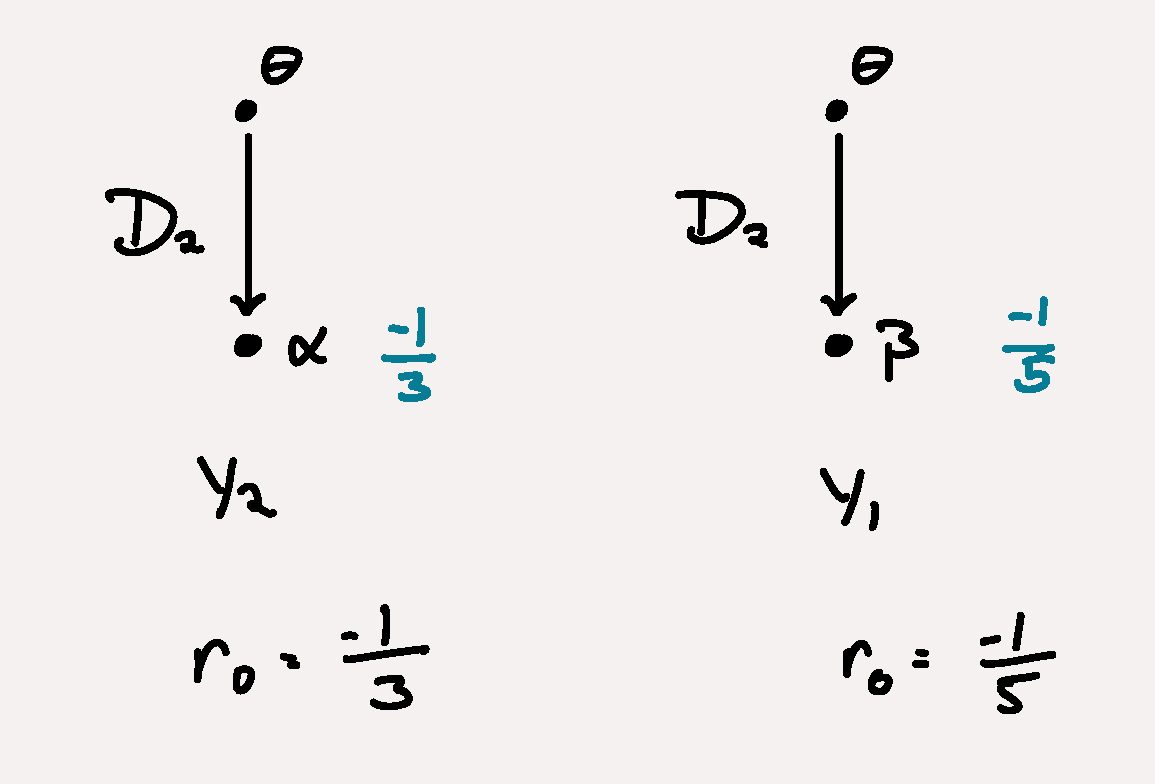
\includegraphics[width=0.5\linewidth]{figures/fig_lec17_towers_example.png}
\end{center}
\end{example}

Here, $r_0$ is measuring the CS displacement of the $D_2$ arrow. The point is that if we pretend $\#$ is $\otimes$, the complex for $Y_1\#Y_2$ looks like:
\begin{center}
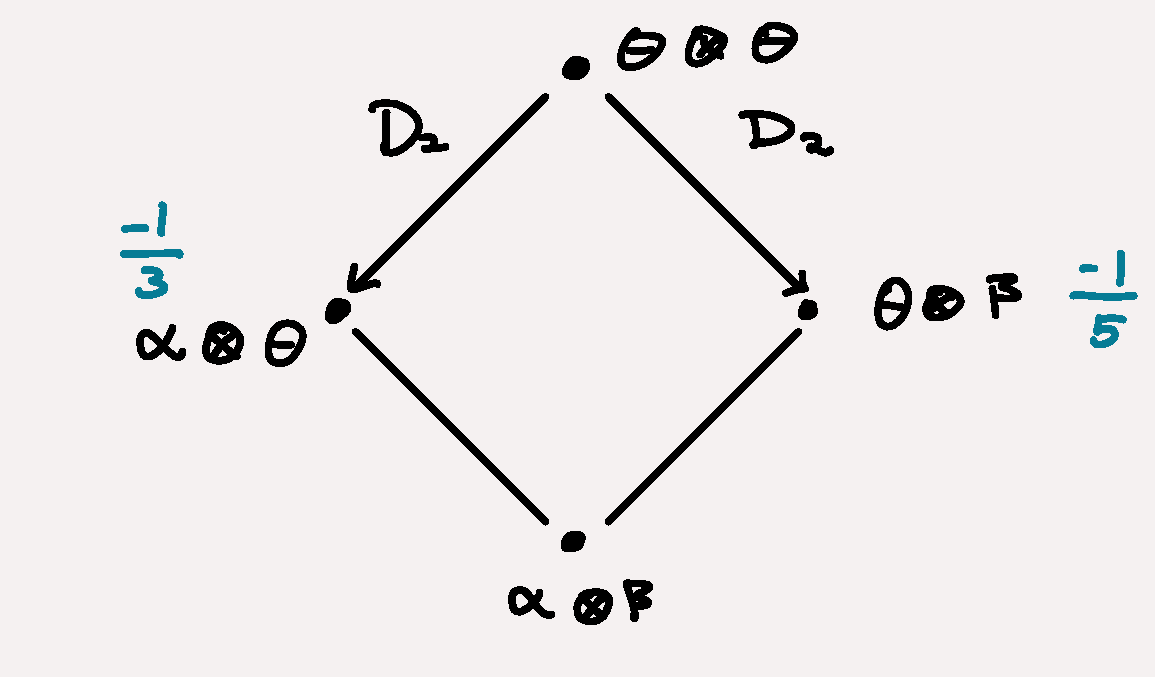
\includegraphics[width=0.4\linewidth]{figures/fig_lec17_diamond.png}
\end{center}
Notice that $D_2(\Theta)$ has $2$ arrows, corresponding to the $2$ summands in the Leibniz rule. Here, it's clear that to kill all the $D_2$'s, you must take the minima of all of the summands.

Unfortunately, it's not actually true, in general, that $\underline{C}(Y_1\#Y_2) = \underline{C}(Y_1)\otimes\underline{C}(Y_2)$. The rough reason is that it turns out that $\underline{C}(Y_1\#Y_2)$ cannot be determined from $\underline{C}(Y_1)$ and $\underline{C}(Y_2)$ alone. To see why, let's look at the potential types of generators of $\underline{C}(Y_1\#Y_2)$:
\begin{itemize}
\item $\Theta\otimes\Theta$ (red $\otimes$ red): this is red,
\item $\alpha\otimes\beta$ (irred $\otimes$ irred),
\item $\Theta\otimes\beta$ (red $\otimes$ irred),
\item $\alpha\otimes\Theta$ (irred $\otimes$ red): these last three are irreducible in the tensor product.
\end{itemize}

The reason why the last two, which are combinations of reducible and irreducible generators, are irreducible in the product is as follows. Recall that generators correspond to $\SU(2)$ representations, and that $\pi_1(Y_1\#Y_2)\cong \pi_1(Y_1)\ast \pi_1(Y_2)$. If we have $\SU(2)$ representations $\rho_1$ and $\rho_2$ of $\pi_1(Y_1)$ and $\pi_1(Y_2)$, and $\rho_1$ has trivial centralizer but $\rho_2$ doesn't, then $\rho_1\ast\rho_2$ also has trivial centralizer. The intuition here is the same as for gauge transformations on the composite cylinder: even if some element commutes with $\rho_2$, it doesn't with $\rho_1$, so it doesn't commute with $\rho_1\ast\rho_2$ either.

The issue arises because $\alpha\otimes\Theta$ and $\Theta\otimes\beta$ are irreducible: there is no reason to expect that there are no flows into/between them! In particular, we should be able to have maps from $\alpha\otimes\beta$ to $\alpha\otimes\Theta$. However, even if there is a $D_1$ map where $D_1(\beta)=\Theta$, in choosing the $\underline{C}$ complex, we threw these out! So you actually need both the $D_1$ and $D_2$ maps of each factor to calculate the $\underline{C}$ complex of the connect sum.

\begin{remark}
Being able to write down an explicit formula for $\underline{C}(Y_1\#Y_2)$ as some tensor product is one motivation for why one may want to try harder to incorporate both $D_1$ and $D_2$ into the differential.
\end{remark}

What salvages this is the fact that there is a cobordism map $\underline{C}(Y_1)\otimes\underline{C}(Y_2) \to \underline{C}(Y_1\#Y_2)$. This cobordism is literally the pair of pants, from $Y_1\sqcup Y_2$ to $Y_1\#Y_2$.
\begin{center}
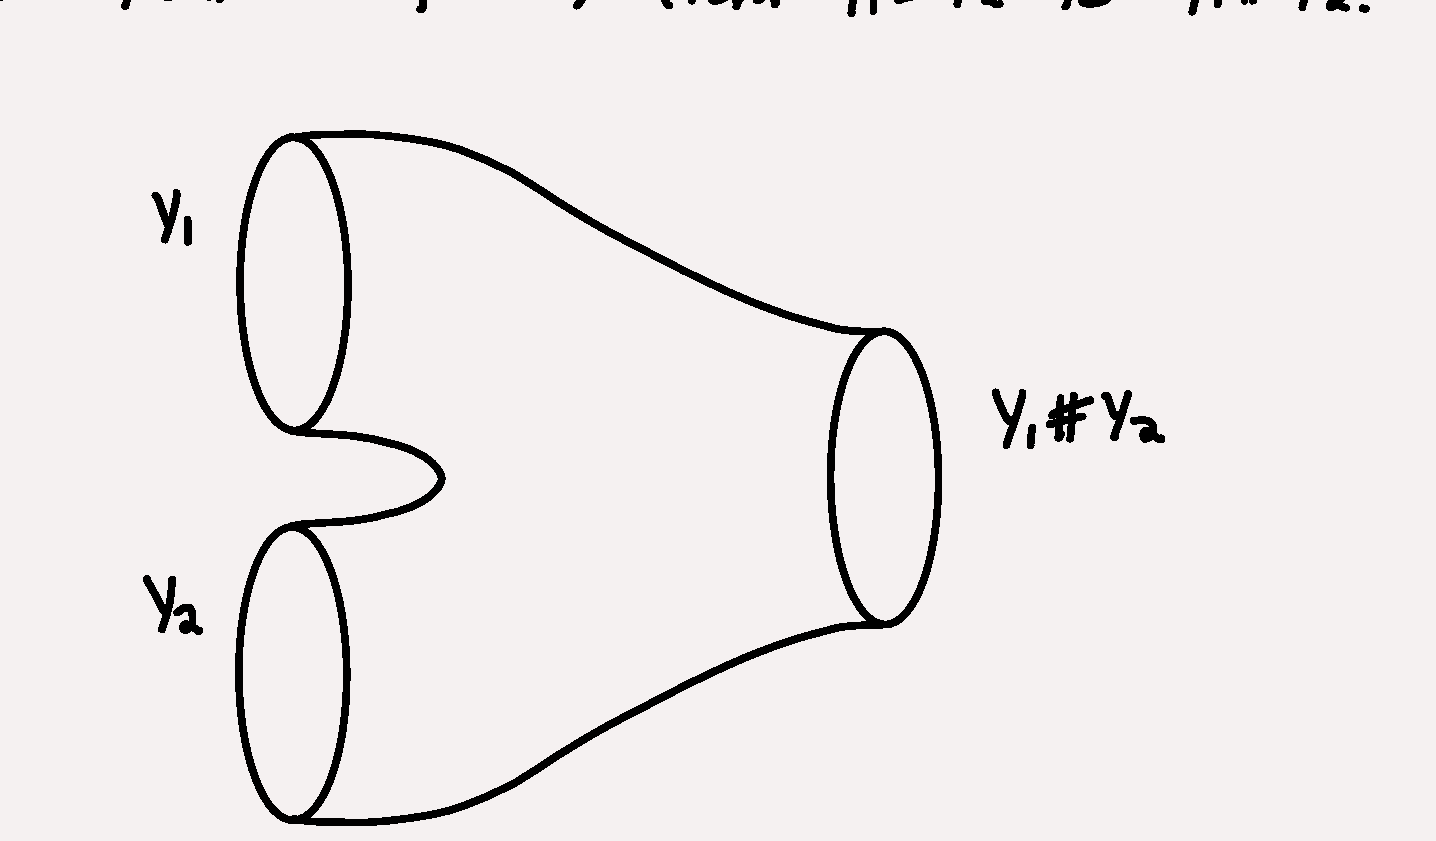
\includegraphics[width=0.55\linewidth]{figures/fig_lec17_pants.png}
\end{center}

Thus far, we've assumed that the $Y$'s are connected, which seems silly to note, but the distinction between connected and disconnected boundary really matters to the gauge group: they're qualitatively different. It turns out that we get bordism maps from disconnected $\to$ connected, but not the other way. But this means that the $r_s$ invariant of the algebraic complex $\underline{C}(Y_1)\otimes\underline{C}(Y_2)$ bounds the $r_s$ invariant of the complex we actually care about, $\underline{C}(Y_1\#Y_2)$.

\begin{question}
Is the inequality always strict?
\end{question}
\noindent\textit{Answer.} No! For example, take $Y_1=-\Sigma(2,3,5)$ and $Y_2=\Sigma(2,3,5)$. Then $Y_1\#Y_2$ is homology cobordant to $S^3$. The $\underline{C}$ complex for each summand looks like

\begin{center}
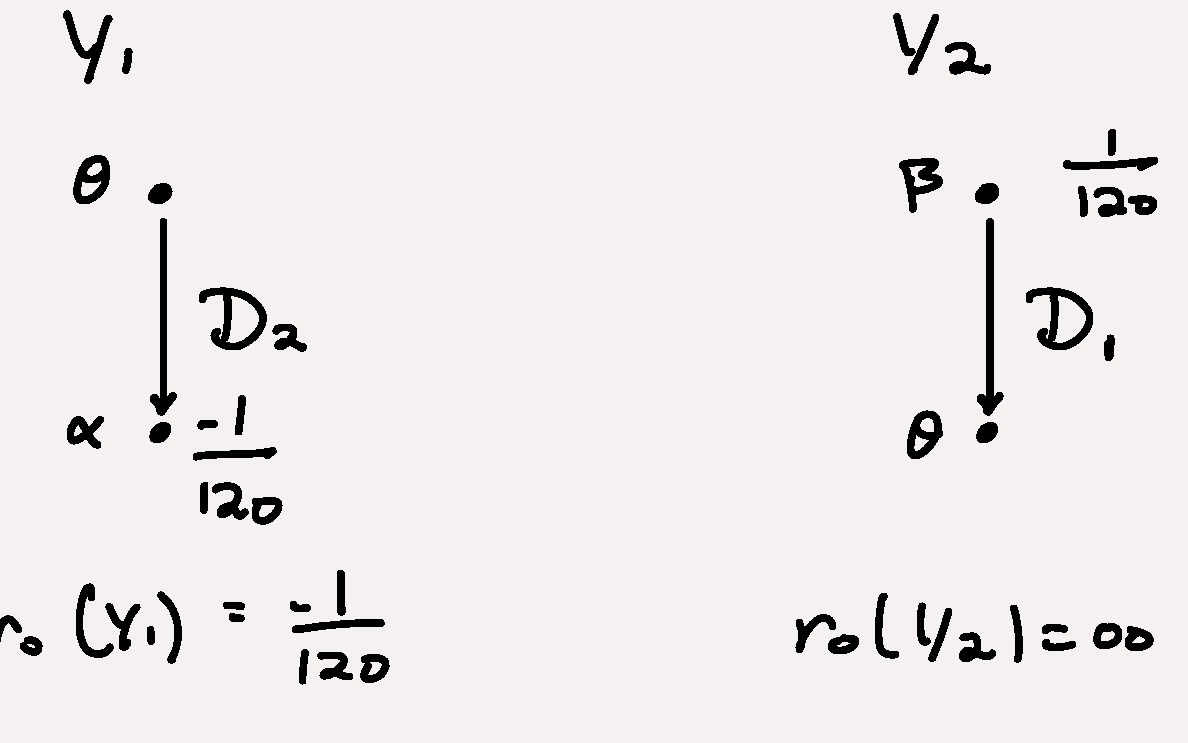
\includegraphics[width=0.6\linewidth]{figures/fig_lec17_towers_counterex.png}
\end{center}

Since $r_s$ is a homology cobordism invariant,
\[
\infty = r_0(S^3) = r_0(Y\#-Y) \geq \min\{r_0(Y), r_0(-Y)\} \geq \min\left\{\frac{1}{120}, \infty\right\} \geq \frac{1}{120}.
\]

We are now prepared to prove the theorem. We'll prove a more general algebraic statement.

\begin{theorem}
Let $\{Y_n\}_{n=1}^\infty$ be a sequence of $\mathbb{Z}\mathrm{HS}^3$'s such that
\begin{enumerate}
\item $\infty > r_0(Y_1) > r_0(Y_2) > \dots$
\item $\infty = r_0(-Y_1) = r_0(-Y_2) = \dots$
\end{enumerate}
Then the $\{Y_n\}_{n=1}^\infty$ are linearly independent in $\Theta^3_{\mathbb{Z}}$.
\end{theorem}

\begin{proof}
Assume not: suppose $\sum_{i\leq m} n_iY_i = 0$ in $\Theta^3_{\mathbb{Z}}$. Then
\[
n_mY_m = \sum_{i<m} n_iY_i \qquad (\text{assume } n_m>0),
\]
so $r_0(n_mY_m) = r_0\left(\sum_{i<m}n_iY_i\right)$. Note that these $n_i$ can be positive or negative. Iterating this inequality, we get that
\[
r_0(n_mY_m) = \dots \geq \min\{r_0(\pm Y_1), r_0(\pm Y_2), \dots\},
\]
where the $+$ or $-$ in each $\pm$ is chosen based on $\mathrm{sign}(n_i)$.

On the other hand, since $Y_m = n_mY_m \# (-n_{m-1})Y_m$,
\[
r_0(Y_m) = r_0\left(n_mY_m \# (-n_{m-1})Y_m\right) \geq \min\{r_0(n_mY_m), r_0(-Y_m)\} \geq \min\{r_0(n_mY_m), \infty\} = r_0(n_mY_m),
\]
since $r_0(-Y_m)=\infty$ by hypothesis. Thus $r_0(Y_m) \geq r_0(n_mY_m)$, so
\[
r_0(Y_m) \geq \min\{r_0(\pm Y_1), r_0(\pm Y_2), \dots\},
\]
which contradicts the initial hypotheses. \qedhere
\end{proof}

The approximate intuition for this result is that small and nonzero CS displacement of $D_2$ cannot lie in the span of large CS displacements.

Does this apply to our situation? Yes! Here's a slick topological argument, which concludes the proof of NST.

\begin{theorem*}[Nozaki-Sato-Taniguchi (\cref{thm:nst})]
Let $k\subseteq S^3$. Denote $Y_n = S^3_{1/n}(k)$, $n>0$. If $[D_2^{Y_1}]\neq 0$, then none of the $Y_n$ are homology cobordant to each other.
\end{theorem*}

\begin{proof}
We only need to show that the conditions of the previous theorem are satisfied. E.g., we need to verify that
\begin{enumerate}
\item $\infty > r_0(Y_1) > r_0(Y_2) > \dots$
\item $\infty = r_0(-Y_1) = r_0(-Y_2) = \dots$
\end{enumerate}

(1) holds from last time: we constructed a $\pi_1=1$ negative-definite cobordism from $Y_{n+1}$ to $Y_n$:

\begin{center}
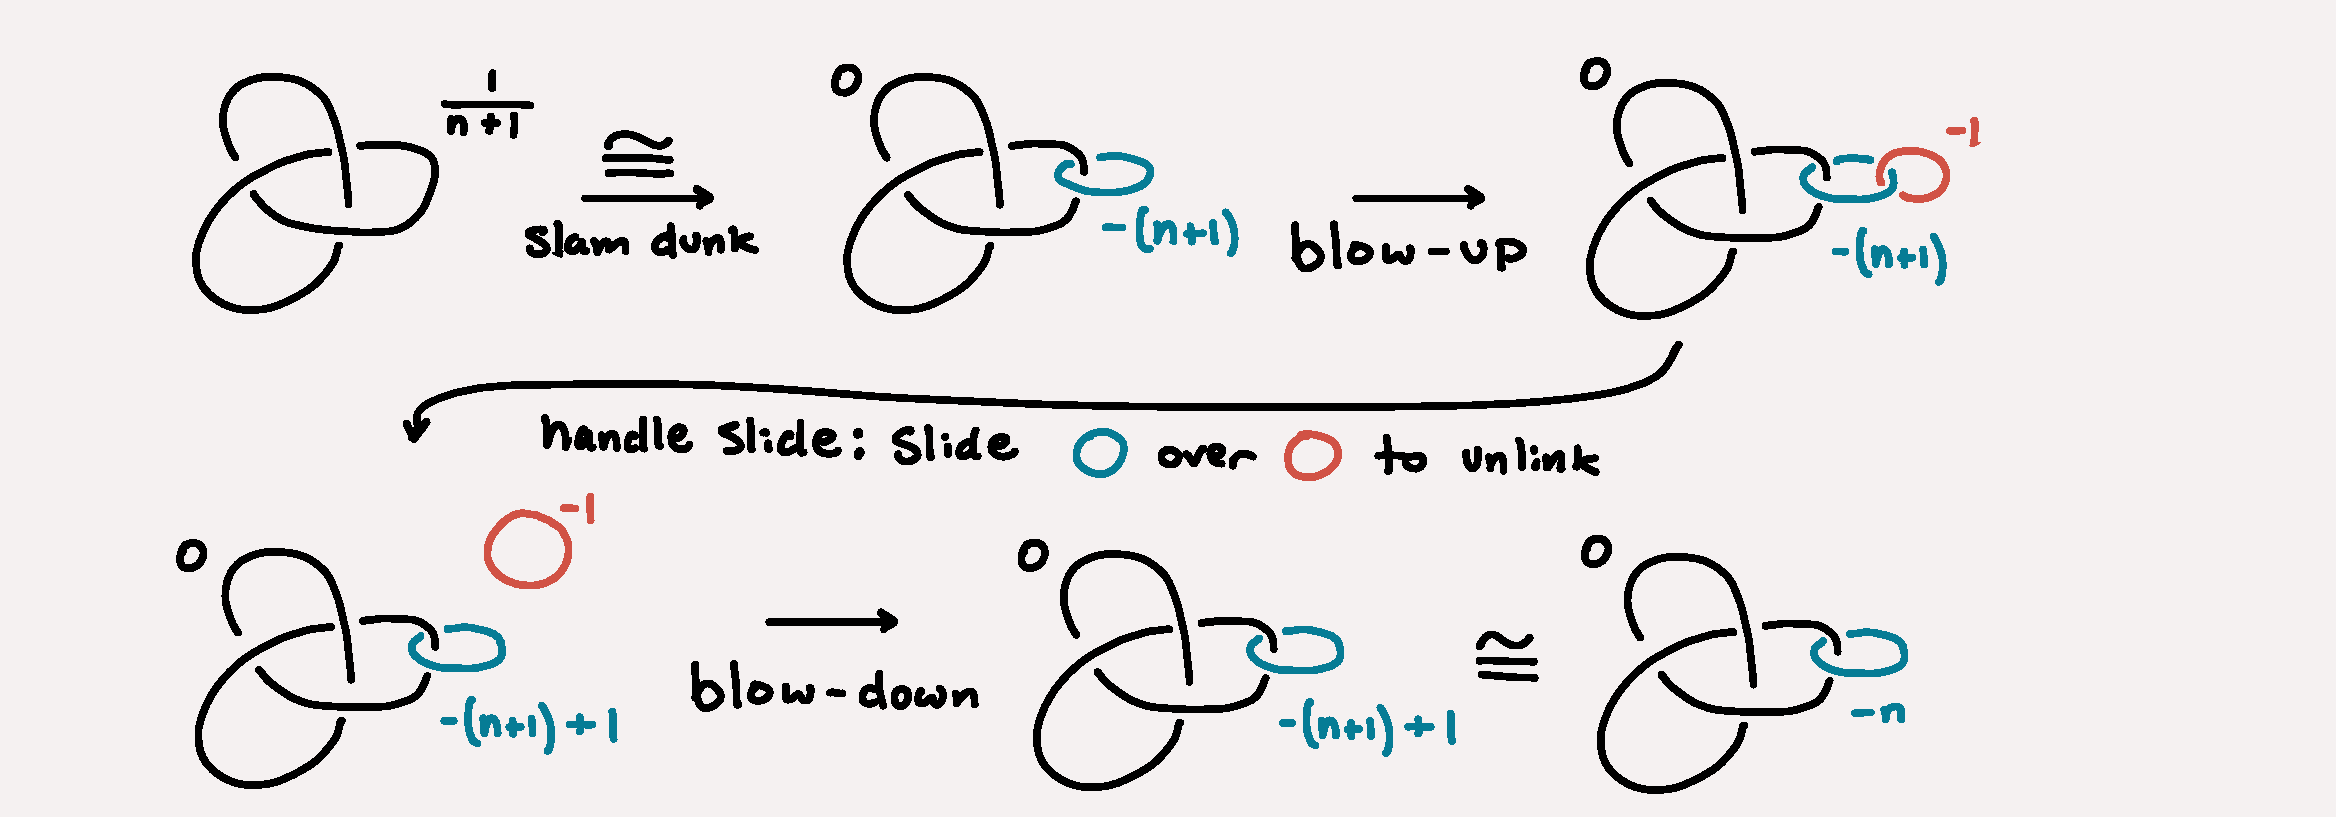
\includegraphics[width=0.9\linewidth]{figures/fig_lec17_kirby_negdef.png}
\end{center}

(2) follows from the fact that $S^3_{1/n}(k)$ bounds a positive-definite manifold if $n>0$ and a negative-definite manifold if $n<0$.

The positive-definite manifold can be constructed as follows ($n>0$):

\begin{center}
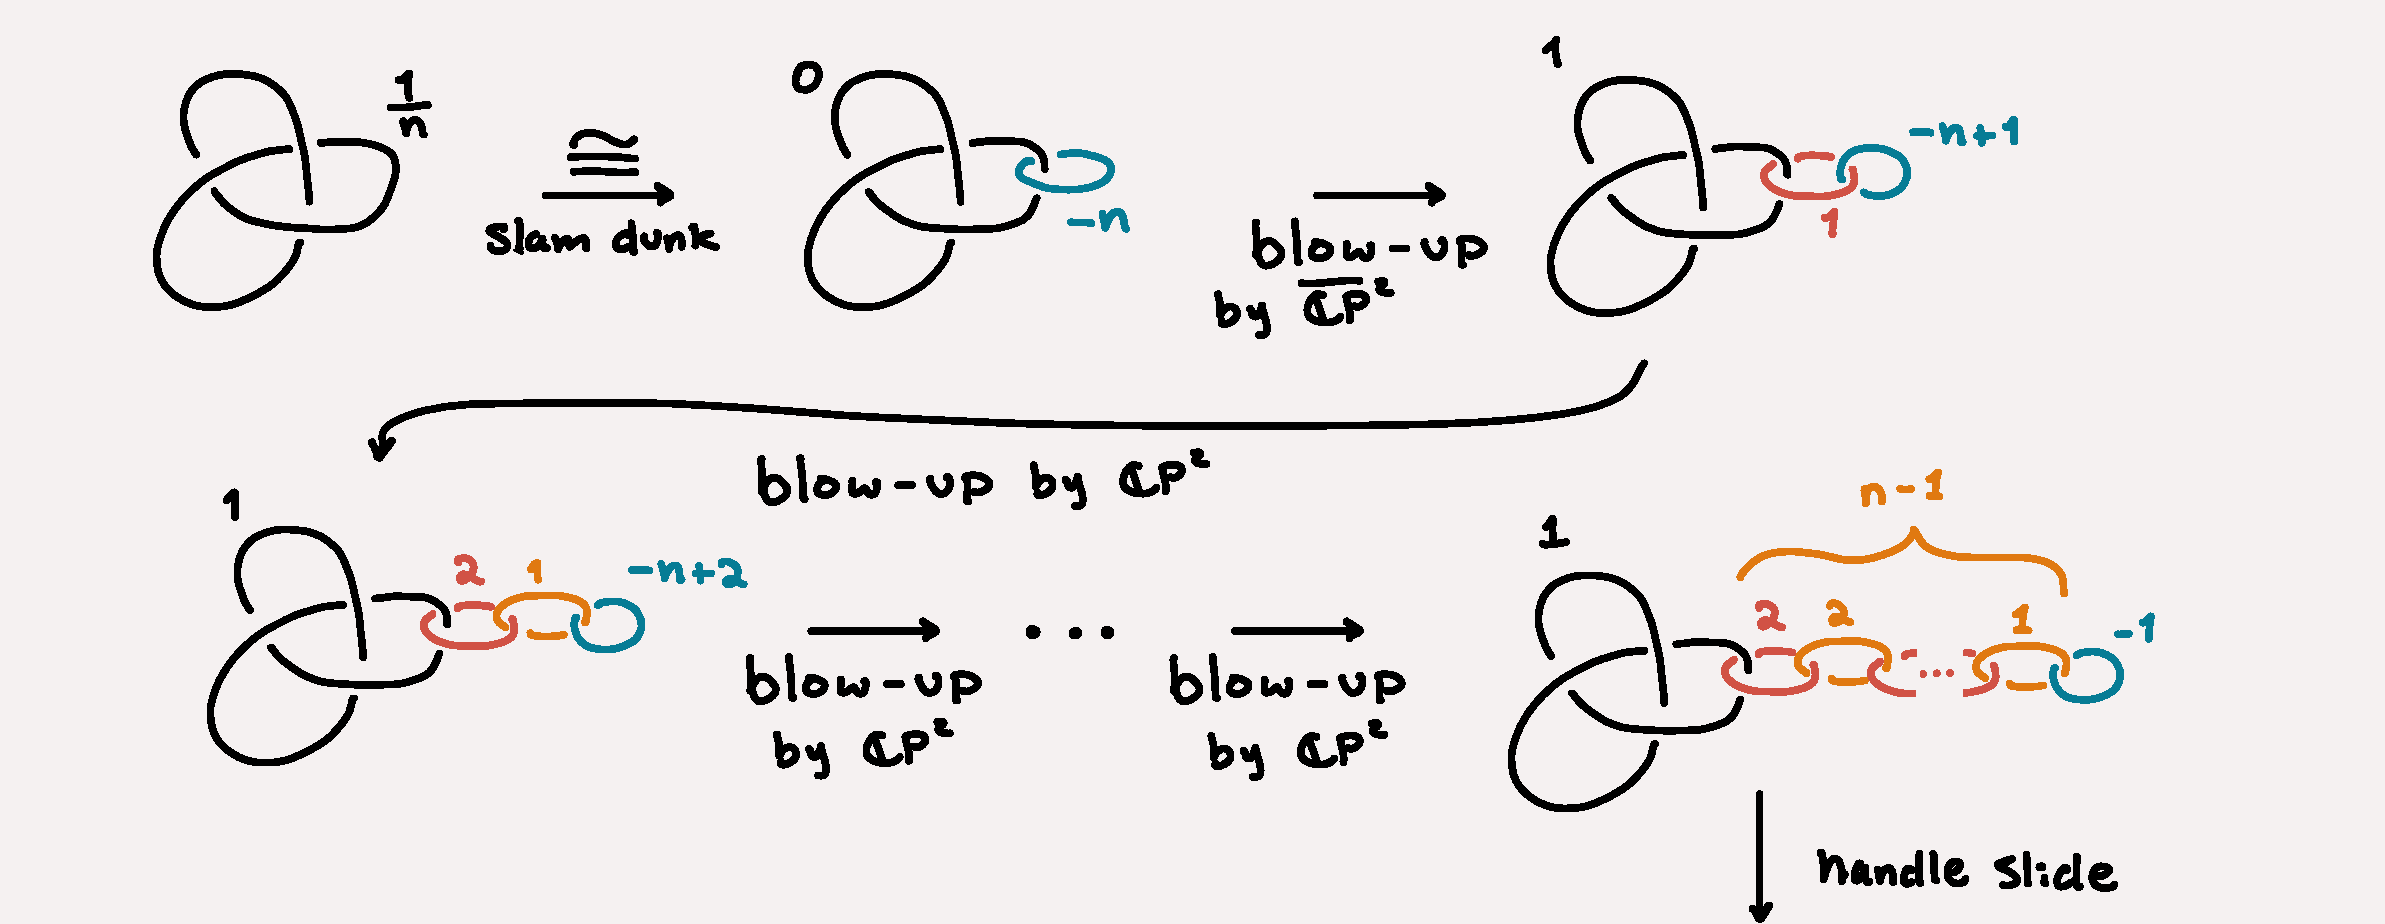
\includegraphics[width=0.9\linewidth]{figures/fig_lec17_kirby_posdef1.png}
\end{center}
\begin{center}
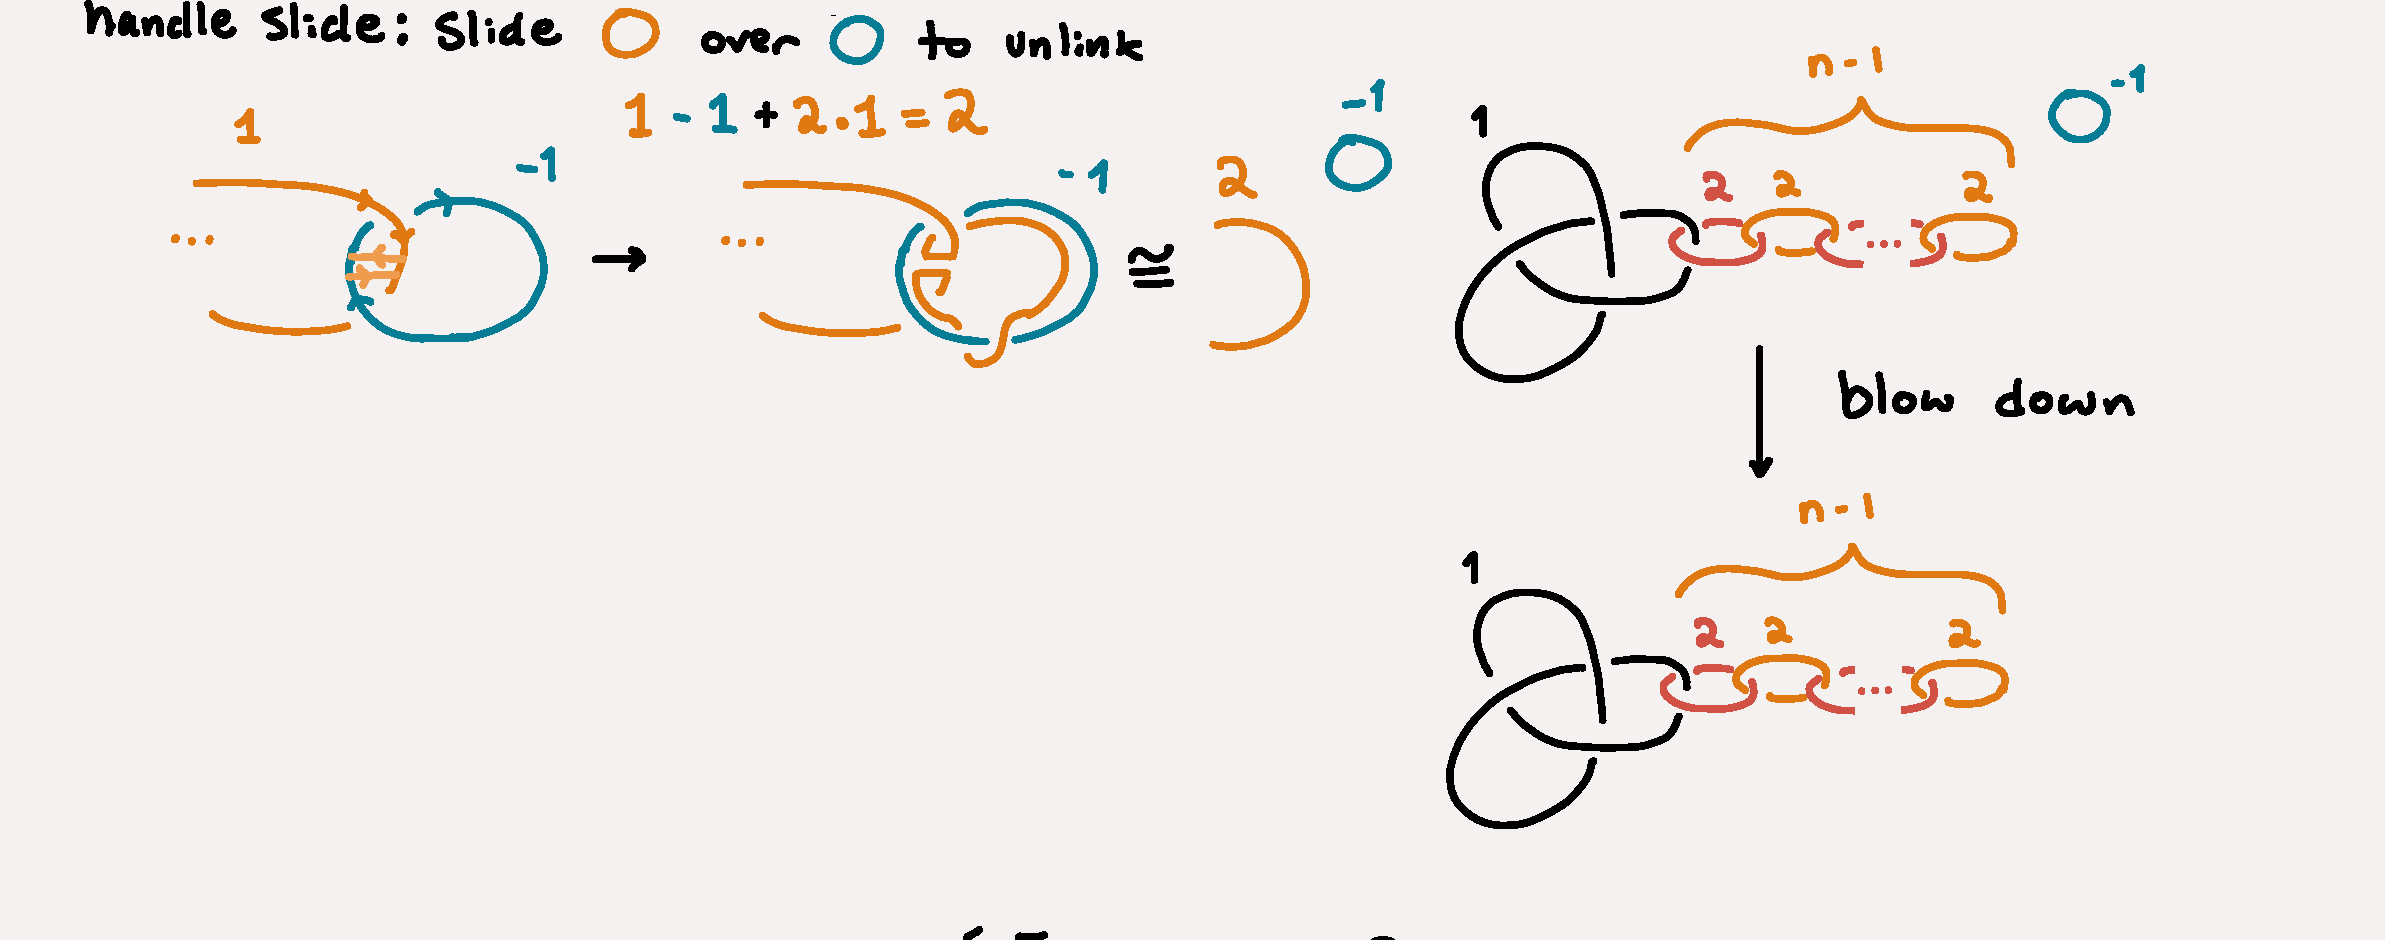
\includegraphics[width=0.9\linewidth]{figures/fig_lec17_kirby_posdef2.png}
\end{center}

The intersection form is

\begin{center}
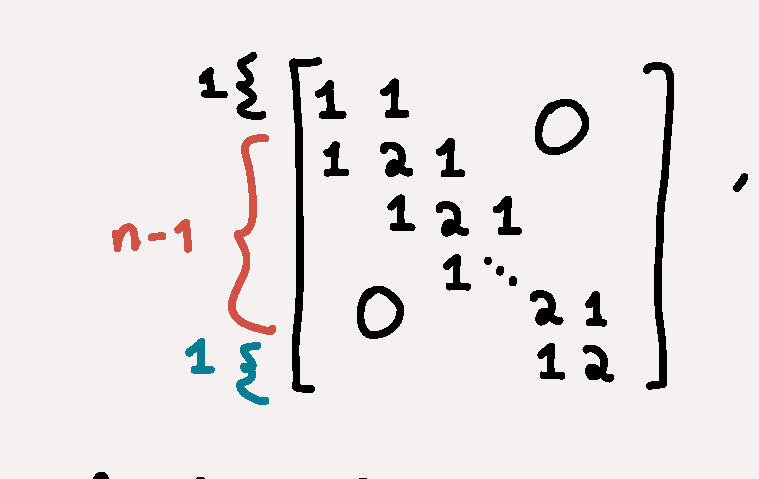
\includegraphics[width=0.35\linewidth]{figures/fig_lec17_intersection_matrix.png}
\end{center}

which we leave to the reader to verify has Smith normal form $\mathrm{Id}$.

The same process can be applied when $n<0$ by blowing up with $\overline{\CP}^2$'s. Since this process gives a negative-definite cobordism from $-Y_n$ to $S^3$, we can conclude that $r_0(-Y_n)=\infty$. \qedhere
\end{proof}

\end{document}
